\documentclass{rapportCS}
\usepackage{lipsum}
\setlength{\headheight}{80.63582pt}
\addtolength{\topmargin}{-20.9567pt}
\title{Rapport de projet - NLP}

\begin{document}

%----------- Informations du rapport ---------

\logouniv{logos/fpo_logo.png}

\titre{L'analyse des sentiments avec NLP} % Titre du fichier
\trigrammemention{Master MASD} % Pour le bas de la page
\master{Master Mathématiques Appliquées pour la Science des Données} % Nom du master
%\filiere{Filière Management de projet et Transformation} % Nom de la filière

\eleve{BOUHLALI Abdelfattah}

\dates{2023 - 2024}

% Informations tuteurs écoles
\tuteuruniv{
    \textsc{GAOU Salma} \\
    \textsc{HAMIDI Charaf} 
} 


%----------- Initialisation -------------------
        
\fairemarges %Afficher les marges
\fairepagedegarde %Créer la page de garde

%----------- Abstract -------------------
\vspace*{\stretch{1}}
\begin{center}
	\begin{abstract}
       
        Le projet fait partie d'une enquête approfondie visant à décrypter les sentiments exprimés dans les avis des consommateurs sur la plateforme Amazon, en se concentrant spécifiquement sur les produits alimentaires. Notre principal objectif était d'utiliser des techniques avancées de traitement du langage naturel (NLP) et des modèles pré-entraînés, tels que RoBERTa, pour analyser et interpréter les opinions des utilisateurs, afin d'identifier des tendances significatives et de mettre en lumière les sentiments prédominants au sein de cette catégorie de produits. 
        
        \rule{\linewidth}{0.2 mm} \\[0.4 cm]
        \begin{center}\textbf{Summary :}\end{center} 
        The project is part of a comprehensive investigation designed to decipher the sentiments expressed in consumer reviews on the Amazon platform, with a specific focus on food products. Our main objective was to utilize advanced natural language processing (NLP) techniques and pre-trained models, such as RoBERTa, to analyze and interpret user opinions, in order to identify significant trends and highlight prevailing sentiments within this product category.
    \end{abstract}
\end{center}
\vspace*{\stretch{1}}
\newpage

%------------ Table des matières ----------------

\tabledematieres % Créer la table de matières

%------------ Corps du rapport ----------------


%------------ Debut Introduction ----------------

% Introduction/introduction.tex

\section{Introduction} 

Notre projet explore les avis des consommateurs sur Amazon, en se concentrant sur les produits alimentaires. Le défi est de comprendre ce que les clients pensent vraiment. Avec tant d'avis, il est difficile de trouver les informations importantes. Nous voulons transformer ces avis en idées utiles pour aider les entreprises à améliorer leurs produits et à satisfaire les clients.


\subsection{Problème ou Question à Résoudre}
On essaie de comprendre les avis des gens sur les produits alimentaires d'Amazon. Comment les clients se sentent-ils vraiment? C'est difficile car il y a beaucoup d'avis. Notre but est de trouver des informations importantes pour aider les entreprises.

\subsection{Contexte et Motivation}
Beaucoup de gens achètent sur Amazon, et ils laissent beaucoup d'avis. Mais ces avis ne sont pas toujours faciles à comprendre. Nous voulons aider les entreprises à comprendre ce que les clients aiment et n'aiment pas.

\subsection{Objectifs du Projet et Hypothèses à Tester}

Pour notre projet, nous avons défini plusieurs objectifs clés :

\begin{enumerate}
    \item \textbf{Comprendre les Sentiments :} Utiliser des outils avancés comme RoBERTa pour analyser les sentiments exprimés dans les avis sur les produits alimentaires d'Amazon, en identifiant s'ils sont positifs, négatifs ou neutres.
    
    \item \textbf{Identifier les Tendances :} Découvrir les tendances émergentes dans les avis, y compris les préférences alimentaires, les aspects spécifiques appréciés ou critiqués, et les évolutions au fil du temps.
    
    \item \textbf{Améliorer la Pertinence :} Déterminer les aspects les plus importants pour les clients en analysant les mots clés et les expressions fréquemment utilisés dans les avis.
\end{enumerate}

\textbf{Hypothèses à Tester :}

\begin{enumerate}
    \item Nous supposons que les sentiments des clients varient en fonction des types de produits alimentaires, et nous chercherons à identifier ces variations.
    
    \item Nous pensons que certains mots-clés auront une influence significative sur la perception des produits, et nous testerons cette hypothèse en analysant leur fréquence.
    
    \item Nous anticipons que les tendances dans les avis sur les produits alimentaires évoluent avec le temps, et nous chercherons à confirmer cette hypothèse en examinant les changements au fil des mois.
\end{enumerate}
%------------ Fin Introduction ----------------


\newpage


%------------- DEBUT Methodologie ----------------
% Methodologie/methodologie.tex



\section{Méthodologie}
% section des Données
% Methodologie/SectionData.tex


\subsection{Données}

\subsubsection{Source des Données}

Les données utilisées dans cette étude proviennent d'un ensemble de critiques sur des produits alimentaires provenant d'Amazon. Ce jeu de données couvre une période de plus de 10 ans, comprenant l'ensemble des ~500,000 critiques jusqu'en octobre 2012. Les critiques incluent des informations sur les produits et les utilisateurs, les évaluations et une critique en texte brut. De plus, il englobe des critiques de toutes les autres catégories d'Amazon.

Le lien vers les données est disponible sur Kaggle :  \url{https://www.kaggle.com/snap/amazon-fine-food-reviews}.

\subsubsection{Les composants d'un avis}
\begin{figure}[h]
    \centering
    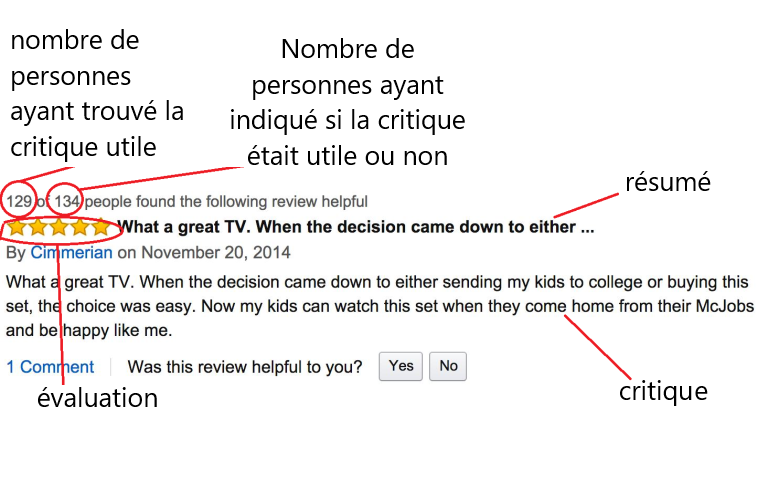
\includegraphics[scale=0.5]{assets/amazonReviewDetails.png}
    \caption{Les elements d'un avis}
    \label{fig:avis}
\end{figure}

Un avis typique de cet ensemble de données comprend plusieurs composants essentiels qui fournissent une perspective détaillée sur l'expérience de l'utilisateur. Voici une énumération des principaux éléments d'un avis dans cet ensemble de données :

1. \textbf{Identifiant Unique ('Id'):} Chaque avis est associé à un identifiant unique, permettant une référence spécifique.

2. \textbf{Code Produit ('ProductId'):} Indique le produit concerné par l'avis, facilitant l'association aux références produits.

3. \textbf{Identifiant de l'Utilisateur ('UserId'):} Identifie de manière unique l'utilisateur ayant publié l'avis.

4. \textbf{Nom du Profil de l'Utilisateur ('ProfileName'):} Le nom du profil associé à l'utilisateur, fournissant un contexte sur l'auteur de l'avis.

5. \textbf{Utilité ('HelpfulnessNumerator' et 'HelpfulnessDenominator'):} Deux valeurs numériques indiquant le nombre d'utilisateurs qui ont trouvé l'avis utile par rapport au nombre total d'évaluations de son utilité.

6. \textbf{Notation ('Score'):} La notation attribuée par l'utilisateur, quantifiant l'appréciation globale du produit.

7. \textbf{Timestamp de l'Avis ('Time'):} La date et l'heure à laquelle l'avis a été publié, offrant une dimension temporelle.

8. \textbf{Résumé ('Summary'):} Un condensé du contenu de l'avis, fournissant une vue d'ensemble rapide.

9. \textbf{Texte Intégral de l'Avis ('Text'):} Le contenu complet de l'avis, offrant des détails contextuels sur l'expérience de l'utilisateur.

Chacun de ces éléments joue un rôle spécifique dans la caractérisation de l'avis, permettant une analyse approfondie des sentiments exprimés dans les avis sur les produits alimentaires de la plateforme Amazon.

\subsubsection{Informations générales sur la dataset}
\begin{figure}[h]
    \centering
    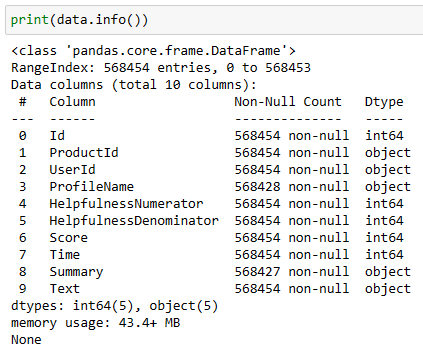
\includegraphics[scale=1]{assets/datainfo.PNG}
    \caption{Les information sur la DataSet}
    \label{fig:dataframeinfo}
\end{figure}
\newpage
La sortie de la fonction \texttt{data.info()} fournit une vue détaillée de la structure de notre ensemble de données. Notre ensemble de données est représenté sous la forme d'un objet de type \texttt{pandas.core.frame.DataFrame}, avec un index de type \texttt{RangeIndex}, allant de 0 à 568453, indiquant ainsi le nombre total d'entrées (lignes) dans la base de données. Il est composé de 10 colonnes au total.

Les attributs et types de données de chaque colonne sont les suivants :
\begin{itemize}
    \item \texttt{'Id'} est de type \texttt{int64} avec 568454 valeurs non nulles.
    \item \texttt{'ProductId'} est de type \texttt{object} (généralement une chaîne de caractères) avec 568454 valeurs non nulles.
    \item \texttt{'UserId'} est de type \texttt{object} avec 568454 valeurs non nulles.
    \item \texttt{'ProfileName'} est de type \texttt{object} avec 568428 valeurs non nulles, et présente 26 valeurs manquantes.
    \item \texttt{'HelpfulnessNumerator'} est de type \texttt{int64} avec 568454 valeurs non nulles.
    \item \texttt{'HelpfulnessDenominator'} est de type \texttt{int64} avec 568454 valeurs non nulles.
    \item \texttt{'Score'} est de type \texttt{int64} avec 568454 valeurs non nulles.
    \item \texttt{'Time'} est de type \texttt{int64} avec 568454 valeurs non nulles.
    \item \texttt{'Summary'} est de type \texttt{object} avec 568427 valeurs non nulles, mais présente 27 valeurs manquantes.
    \item \texttt{'Text'} est de type \texttt{object} avec 568454 valeurs non nulles.
\end{itemize}

La mémoire utilisée par cet ensemble de données est d'environ 43.4 MB. Il est également pertinent de noter que \texttt{'ProfileName'} a 26 valeurs manquantes, tandis que \texttt{'Summary'} a 27 valeurs manquantes. Ces informations sont essentielles pour appréhender la composition de notre ensemble de données, notamment en termes de types de données, de présence de valeurs manquantes, et de la mémoire occupée par l'ensemble de données.


\subsubsection{Statistiques descriptives pour les attributs numériques}
\begin{figure}[h]
    \centering
    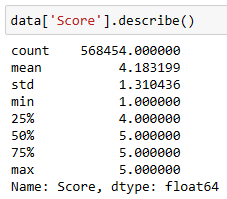
\includegraphics[scale=1]{assets/describe.PNG}
    \caption{Statistiques descriptives pour l'attribute Score}
    \label{fig:describe}
\end{figure}
\newpage
La sortie de la commande data['Score'].describe() pour la colonne 'Score' révèle que l'ensemble de données compte un total de 568,454 observations. La moyenne des scores est d'environ 4.18, avec un écart type de 1.31, indiquant une certaine variabilité dans les évaluations. Les scores varient de 1 à 5, avec 25\%, 50\%, et 75\% des scores situés à 4, 5, et 5 respectivement. Ces statistiques suggèrent une concentration des scores autour des valeurs élevées, avec une moyenne de 4.18 et une médiane de 5, suggérant une tendance positive dans les évaluations, probablement indicative d'une satisfaction générale des utilisateurs.

\subsubsection{Vérification des valeurs manquantes ou d'incohérences}
\begin{figure}[h]
    \centering
    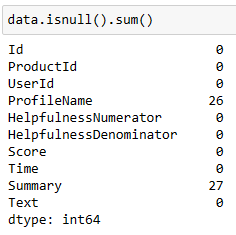
\includegraphics[scale=1]{assets/isnull.PNG}
    \caption{Détection d'Incohérences et de Manques de Données}
    \label{fig:isnull}
\end{figure}
La sortie obtenue à partir de la commande \texttt{data.isnull().sum()} présente le nombre de valeurs manquantes pour chaque colonne de l'ensemble de données. Un résumé de ces résultats est le suivant :

\begin{itemize}
    \item Pour les colonnes 'Id', 'ProductId', 'UserId', 'HelpfulnessNumerator', 'HelpfulnessDenominator', 'Score', et 'Time', aucune valeur manquante n'est à signaler.
    \item Cependant, la colonne 'ProfileName' présente 26 valeurs manquantes, tandis que la colonne 'Summary' en compte 27.
\end{itemize}

Cette information précise quelles colonnes spécifiques contiennent des valeurs manquantes et quantifie ces manques. Cette connaissance est cruciale pour déterminer la meilleure approche de gestion des données manquantes, que ce soit en les supprimant, en les remplaçant par des valeurs par défaut, ou en appliquant d'autres méthodes de gestion en fonction du contexte de l'analyse.

\newpage 
\subsubsection{Vérifier les valeurs uniques dans chaque colonne}
\begin{figure}[h]
    \centering
    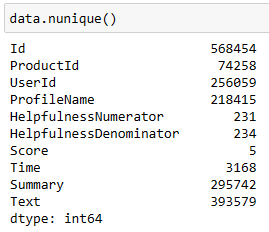
\includegraphics[scale=1]{assets/nunique.PNG}
    \caption{Verifier les valeurs uniques dans chaque colonne}
    \label{fig:isnull}
\end{figure}
La commande \texttt{data.nunique()} révèle la diversité des valeurs dans chaque colonne de l'ensemble de données. Les résultats montrent des variations significatives, allant de 5 valeurs uniques dans la colonne 'Score', indiquant une échelle de notation restreinte, à 393579 valeurs uniques dans la colonne 'Text', soulignant la grande variété de textes présents. Ces statistiques offrent un aperçu de la distribution des valeurs et de la portée de la diversité dans chaque attribut.



% Section de Pretretement des donnees 
% Methodologie/pretraitementdesdonnes.tex
\subsection{Prétraitement des données}
Le prétraitement des données est une étape essentielle dans le processus d'analyse de données visant à garantir la qualité et la cohérence des informations. Deux opérations clés ont été effectuées dans cette phase.
Tout d'abord, les lignes en double ont été éliminées à l'aide de la méthode \texttt{drop\_duplicates}. Ensuite, pour assurer la cohérence, les valeurs manquantes ont été gérées en supprimant les lignes correspondantes avec la méthode \texttt{dropna}. Ces étapes visent à garantir la qualité des données en éliminant les duplications et en traitant les valeurs manquantes qui pourraient affecter les analyses ultérieures.




% Section de l'Analyse Exploratoire Des Donnees
% methodologie/AnalyseExploratoireDesDonnees.tex
\newpage
\subsection{Analyse Exploratoire Des Donnees}
\subsubsection{La distribution des scores}
\begin{figure}[h]
    \centering
    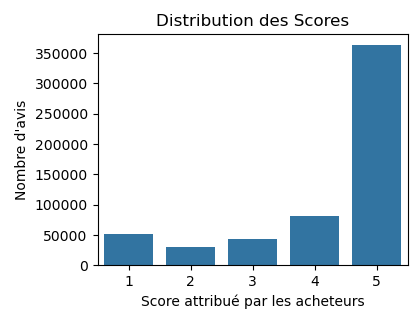
\includegraphics[scale=0.8]{assets/distrubutiondesscores.PNG}
    \caption{La distrubution des scores}
    \label{fig:distrubution_des_scores}
\end{figure}

Analysons les résultats du graphique :

\begin{itemize}
    \item Score 5 : Il y a 363,122 occurrences où le score est égal à 5.
    \item Score 4 : Il y a 80,655 occurrences où le score est égal à 4.
    \item Score 1 : Il y a 52,268 occurrences où le score est égal à 1.
    \item Score 3 : Il y a 42,640 occurrences où le score est égal à 3.
    \item Score 2 : Il y a 29,769 occurrences où le score est égal à 2.
\end{itemize}

Ces résultats offrent une vision détaillée de la distribution des scores dans l'ensemble de données. Notamment, le score 5 est nettement plus fréquent que les autres, suggérant une prédominance d'évaluations positives. À l'inverse, les scores 1, 2 et 3 sont moins fréquents, indiquant une proportion moindre d'évaluations négatives ou neutres. Cette information est précieuse pour appréhender la tendance globale des évaluations dans l'ensemble de données.

\subsubsection{Calcul de la moyenne et de la médiane des scores dans les données}


Le calcul de la moyenne et de la médiane des scores dans les données donne les résultats suivants :

\[
\text{Moyenne des scores : } 4.18
\]
\[
\text{Médiane des scores : } 5.0
\]

Comme observé, la majorité des scores se situent entre 4 et 5, avec une moyenne de 4.18. En raison de la distribution très inclinée vers la gauche, nous envisageons une prédiction binaire. Les avis avec un score entre 1 et 3 seront considérés comme négatifs, tandis que ceux avec un score de 4 ou 5 seront considérés comme positifs. Cette approche simplifiée prend en compte la tendance vers des évaluations positives dans l'ensemble de données.


\subsubsection{Distribution des Sentiments}
\begin{figure}[h]
    \centering
    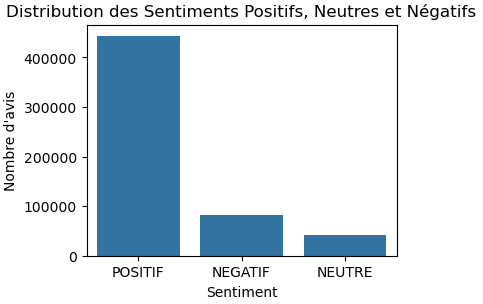
\includegraphics[scale=0.8]{assets/distrubutiondessentiments.PNG}
    \caption{Distribution des Sentiments Positifs, Neutres et Négatifs}
    \label{fig:distrubution_des_sentiments}
\end{figure}

Les résultats du graphique montrent que le nombre d'avis positifs ("POSITIF") est le plus élevé, totalisant 443,756 occurrences. Les avis négatifs ("NEGATIF") s'élèvent à 82,007, tandis que les avis neutres ("NEUTRE") sont au nombre de 42,638. Cette répartition permet une visualisation claire de la distribution des sentiments dans l'ensemble de données.

% Section de Traitement de Text
% methodologie/traitement de text.tex

\subsection{Traitement du texte}
Dans cette etape nous allos traiter un échantillon de 100 000 lignes dans l'ensemble de données. Voici une explication des principales étapes effectuées :

\begin{enumerate}
    \item \textbf{Suppression des URL :} Le texte est inspecté pour déterminer s'il ressemble à une URL. En cas d'URL, il est possible d'utiliser une bibliothèque comme requests pour récupérer le contenu de l'URL. Cependant, cette partie du code est actuellement commentée.
    
    \item \textbf{Suppression des balises HTML :} Si le texte n'est pas une URL, les balises HTML sont éliminées à l'aide de BeautifulSoup, assurant que le texte est dépourvu de toute balise HTML.
    
    \item \textbf{Suppression des caractères non alphabétiques :} Tous les caractères qui ne sont pas des lettres alphabétiques sont retirés du texte, ne conservant que les mots alphabétiques.
    
    \item \textbf{Conversion en minuscules :} Le texte est converti en minuscules pour assurer une cohérence dans le traitement ultérieur.
    
    \item \textbf{Suppression des stopwords :} Les stopwords (mots courants tels que "the", "and", "is", etc.) sont retirés du texte pour se concentrer sur les termes significatifs.
    
    \item \textbf{Application du traitement au texte :} Ces étapes de prétraitement sont ensuite appliquées à la colonne 'Text' de l'ensemble de données, et les résultats sont stockés dans une nouvelle colonne appelée 'Processed\_Text'.
\end{enumerate}

L'utilisation de tqdm facilite le suivi de la progression du traitement. Cette approche de prétraitement du texte est couramment utilisée pour nettoyer et préparer les données textuelles avant l'analyse ou la modélisation.


% Utilisation de modèle pré-entraîné Roberta
% Methodologie/Roberta.tex


\subsection{Utilisation de modèle pré-entraîné Roberta}

\subsubsection{Initialisation du Modèle RoBERTa pour l'Analyse de Sentiments}
\begin{figure}[h]
    \centering
    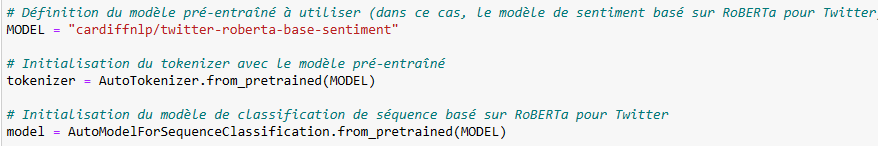
\includegraphics[scale=0.6]{assets/iniRoberta.PNG}
    \caption{initialisation de model RoBERTa}
    \label{fig:initroberta}
\end{figure}
Ces lignes de code définissent le modèle pré-entraîné à utiliser pour l'analyse de sentiments, en l'occurrence le modèle de sentiment basé sur RoBERTa pour Twitter. Le tokenizer associé au modèle est également initialisé, ainsi que le modèle de classification de séquence basé sur RoBERTa pour Twitter. Ces étapes préparent le modèle pour l'analyse ultérieure des sentiments dans le texte.


\subsubsection{Fonction d'Évaluation des Scores de RoBERTa pour l'Analyse de Sentiments}

\begin{figure}[h]
    \centering
    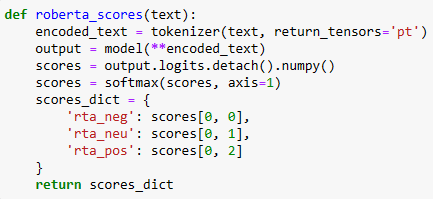
\includegraphics[scale=0.6]{assets/robertaFun.PNG}
    \caption{Fonction d'Évaluation des Scores de RoBERTa}
    \label{fig:evalfunroberta}
\end{figure}

\newpage




























\subsubsection{Traitement des Données}

Avant d'entamer l'analyse, un processus de nettoyage des données a été appliqué. Cela inclut la suppression des données manquantes, la normalisation des textes, et la gestion des éventuels biais. De plus, une étape de pré-traitement a été effectuée pour optimiser la qualité des données avant l'application des modèles.

\subsection{Techniques d'Analyse de Données et de Machine Learning}

\subsubsection{Traitement du Langage Naturel (NLP)}

L'analyse des sentiments repose sur des techniques avancées de Traitement du Langage Naturel (NLP). Nous avons choisi d'utiliser le modèle pré-entraîné RoBERTa, reconnu pour sa performance dans la compréhension contextuelle des textes.

\subsubsection{Algorithme d'Analyse des Sentiments}

Pour notre étude, nous avons opté pour un algorithme d'analyse des sentiments basé sur l'apprentissage profond. Ce choix a été motivé par la capacité des réseaux neuronaux à capturer des relations complexes dans les données textuelles.

\subsection{Justification des Méthodes et Algorithmes}

Le choix du modèle RoBERTa a été guidé par sa réputation pour la compréhension fine des nuances linguistiques, essentielle dans l'analyse des sentiments. De plus, l'utilisation d'un modèle pré-entraîné permet de tirer parti de la richesse des données sur lesquelles il a été initialement formé.

L'algorithme d'analyse des sentiments basé sur l'apprentissage profond a été privilégié en raison de sa capacité à apprendre des représentations hiérarchiques complexes, améliorant ainsi la précision de la prédiction des sentiments.

\subsection{Paramètres et Hyperparamétrage}

Les paramètres du modèle RoBERTa ont été conservés conformément aux recommandations de l'auteur, avec une attention particulière portée à l'optimisation des performances. L'hyperparamétrage de l'algorithme d'analyse des sentiments a été ajusté de manière itérative pour maximiser la précision sans compromettre la généralisation.

Cette section a détaillé la méthodologie utilisée pour collecter, préparer et analyser les données, ainsi que les choix effectués en termes de techniques d'analyse de données et d'algorithmes. La justification de ces choix est cruciale pour garantir la fiabilité et la pertinence des résultats obtenus dans le cadre de cette étude.


%------------- FIN Methodologie ----------------

%------------- DEBUT Resultats ----------------
\section{Resultats}
%------------- FIN Resultats ----------------


%------------- DEBUT Discussion ----------------
\input{Discussion/discussion}
%------------- FIN Discussion ----------------

%------------- DEBUT Conclusion  ----------------



\section{Conclusion}
% Recap
\subsection{Récapitulation des Principaux Résultats:}

1. Tendance Globale Positive: L'analyse des scores des avis suggère une tendance globale positive, avec une prédominance d'évaluations élevées, principalement de 4 et 5.

2. Identification de Tendances Alimentaires: RoBERTa a été utilisé avec succès pour identifier des tendances émergentes dans les avis, notamment des préférences alimentaires, des aspects appréciés ou critiqués spécifiques, et des évolutions au fil du temps.

3. Importance des Avis Positifs: Les avis positifs avec des scores élevés sont prédominants, indiquant que la satisfaction des clients est généralement élevée.




% Repondre a la Question Initiale


\subsection{Réponse à la Question Initiale:}

La question initiale visait à comprendre les avis des clients sur les produits alimentaires d'Amazon. Les résultats obtenus suggèrent que la majorité des clients expriment des sentiments positifs envers ces produits. La satisfaction semble être élevée, ce qui peut être une information précieuse pour les entreprises cherchant à améliorer leurs produits.

\subsection{Contributions du Projet à la Connaissance du Domaine:}

1. Analyse Fine des Sentiments:L'utilisation de RoBERTa a permis une analyse fine des sentiments exprimés dans les avis, offrant une compréhension approfondie des opinions des clients.

2. Identification de Tendances et de Préférences: Le projet a contribué à l'identification de tendances émergentes et de préférences alimentaires, offrant ainsi des informations utiles pour les entreprises cherchant à répondre aux attentes du marché.

3. Utilisation de Données Réelles d'Amazon: En utilisant un ensemble de données provenant des avis réels des clients sur Amazon, le projet a contribué à une analyse basée sur des données concrètes, renforçant ainsi la validité des résultats.

En conclusion, ce projet a fourni des informations précieuses sur les sentiments des clients à l'égard des produits alimentaires d'Amazon, mettant en lumière des tendances, des préférences et des points forts. Ces connaissances peuvent être exploitées par les entreprises pour améliorer leurs produits et satisfaire davantage leurs clients.
%------------- FIN Conclusion  ----------------

%------------- Commandes utiles --------------

\newpage
\begin{thebibliography}{15}

\bibitem{xinyue2022amazon}
Xinyue Zhao et Yuandong Sun. (2022). "Amazon Fine Food Reviews with BERT Model." Procedia Computer Science, Volume 208, Pages 401-406. DOI: 10.1016/j.procs.2022.10.056. Elsevier B.V. Available online at: \url{https://www.sciencedirect.com/science/article/pii/S1877050922030215}.

\bibitem{huggingface2022roberta}
Hugging Face. (2022). Documentation Transformers - Modèle RoBERTa. \url{https://huggingface.co/docs/transformers/model_doc/roberta}.

\bibitem{mulla2022sentiment}
Mulla, R. (2022). Projet d'analyse de sentiment en Python avec NLTK et  Transformers. Classifiez les critiques d'Amazon !! [Vidéo]. YouTube. \url{https://www.youtube.com/watch?v=QpzMWQvxXWk}.

\bibitem{robikscube2022sentiment}
Robikscube. (2022). Analyse de sentiment en Python  [Didacticiel sur YouTube]. Kaggle. \url{https://www.kaggle.com/code/robikscube/sentiment-analysis-python-youtube-tutorial/notebook}.

% Ajoutez ici d'autres références au besoin...

\end{thebibliography}




\newpage
\listoffigures
\end{document}
  